\documentclass[a4paper,oneside,12pt]{article}

%---------------------------
% Header
%---------------------------
\usepackage{longtable,geometry}
\usepackage[frenchb]{babel}
\usepackage[utf8]{inputenc}
\usepackage[T1]{fontenc}
\usepackage[babel]{csquotes}
\usepackage{graphicx}
\usepackage[absolute]{textpos}
\usepackage{fancyhdr}
\usepackage{pslatex}
\usepackage[toc,page]{appendix} 

% Header 
\pagestyle{fancy}
\fancyhf{}
\lhead[\thepage]{\rightmark} 
\rhead[\leftmark]{\thepage}
\cfoot[\thepage]{- \thepage ~-} 

\MakeAutoQuote{«}{»}
\textwidth 14.8cm
\oddsidemargin 0.0in 
\textheight 22.94cm 
\setlength{\skip\footins}{1cm}

%---------------------------
% Document
%---------------------------
\begin{document}
%---------------------------
% Title
%---------------------------
\begin{titlepage}
\begin{center}

\includegraphics[scale=.4]{img/logos/logo-mymed} ~~~~~~~~~~~~~~~~~~~~~~~~~~~~~~~~~~~~~~~~~~~~~~~~~~~~~~~~~~~~~~~~~~~

\includegraphics[scale=.25]{img/logos/Logo_INRIA}
\vskip 1.5cm
Trustworthy Global Computing 2010
\vskip 1cm
{\Huge\bfseries Réseau social Pair a Pair spécialisé dans le co-voiturage}
\vskip 1cm
Supported by AEOLUS FP6-IST-15964-FET Proactive and DEUKS JEP-41099 TEMPUS.
\vskip 1.5cm
\end{center}
2009 LogNet Team - INRIA Sophia Antipolis - Méditerranée , France:\\
Laurent Vanni: laurent.vanni@sophia.inria.fr\\
Luigi Liquori: luigi.liquori@sophia.inria.fr\\
Vincenzo Ciancaglini: vincenzo.ciancaglini@sophia.inria.fr
\begin{center}
\vskip 0.5cm
24 decembre 2009
\vskip 1cm
Résumé\\
\end{center}
{\em Ce document présente un prototype de réseau de covoiturage, adapté et optimisé pour une zone géographique précise. Il utilise une architecture Pair a Pair, est constitue un exemple d'utilisation du protocole Synapse\footnote{Protocole développé par l'équipe Lognet - INRIA Sophia Antipolis - Méditerranée , France : http://www-sop.inria.fr/teams/lognet/synapse/}}
\vskip 2cm

\includegraphics[scale=0.7]{img/logos/cnrs} ~~~~~~~~~~~~~~~~~~~~~~

\includegraphics[scale=0.3]{img/logos/logo-i3s}  ~~~~~~~~~~~~~~~~~~~~~~

\includegraphics[scale=0.3]{img/logos/epu}
\end{titlepage} 
\clearpage

%---------------------------
% Table of contents
%---------------------------
\tableofcontents \clearpage

%---------------------------
% Intro
%---------------------------
\section{Introduction}
\textbf{Pré-requis:} Ce prototype ne prend pas en compte le \% de personnes utilisant les transports en communs.\\

Considérons trois centres de recherches et développements géographiquement très proches:
\begin{itemize}
\item L'école Polytech'Nice-Sophia
\item L'INRIA - Sophia Antipolis - Méditerranée , France
\item Le laboratoire i3s du CNRS \\
\end{itemize}

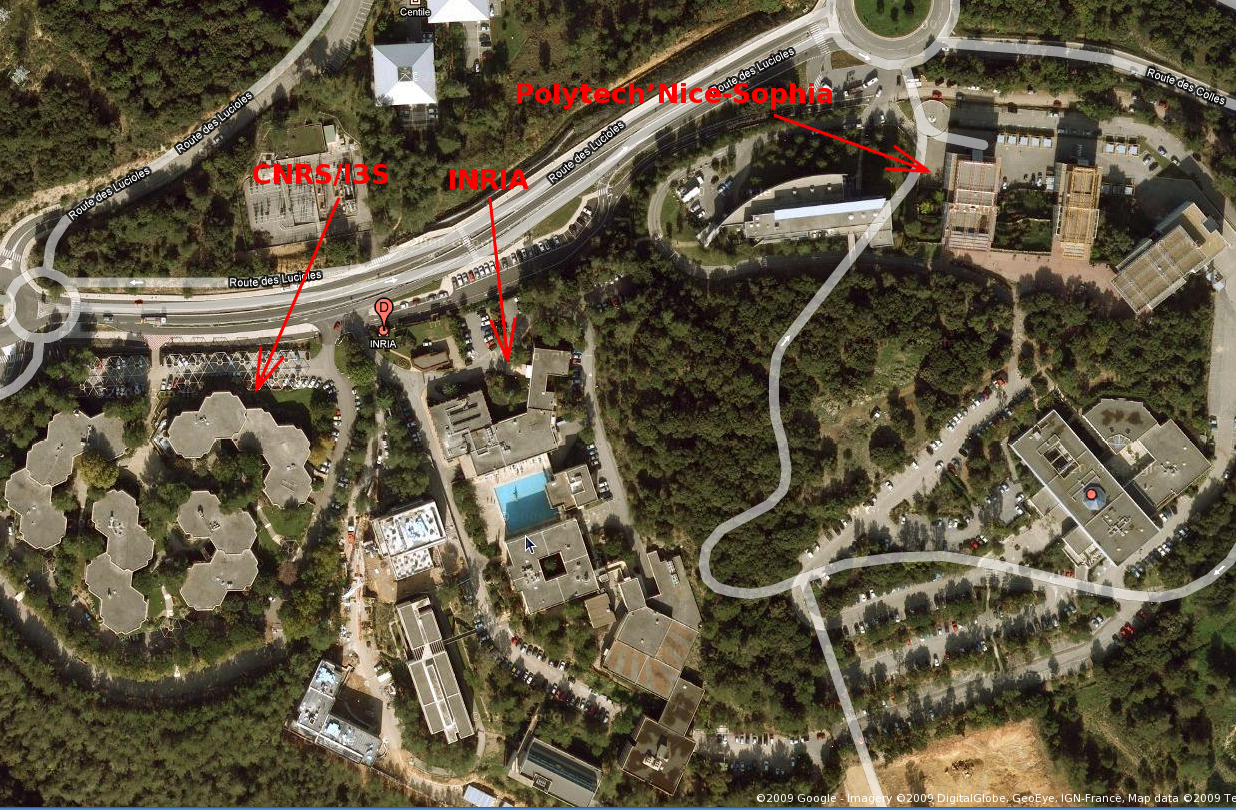
\includegraphics[scale=0.35]{img/screenshot/geolock} \\

Parmi ces 3 centres, on peut distinguer 2 types de personnes:
\begin{itemize}
\item Les Étudiants: \\
	Polytech'Nice-Sophia accueille près de \textbf{1.000 élèves} qui suivent les formations offertes dans cinq grands domaines scientifiques et technologiques  - Électronique, Informatique, Mathématiques appliquées, Génie biologique et Ingénierie de l'eau
\item Les Autres: \\
	Chercheurs, enseignants chercheurs, doctorant, ingénieurs, personnels administratifs, ...)
	repartis entre l'INRIA, le CNRS et l'école Polytech'Nice-Sophia (\textbf{environs 500 personnes}) \\
\end{itemize} 

Le cas critique pour cette zone géographique de sophia-antipolis, serai que toutes ces personnes possèdent une voiture sans jamais faire de covoiturage: environs 1500 voitures mobilisées tous les jours!
A l'inverse, le cas idéal serai que tout le monde propose de faire du co-voiturage, on obtiendrait pour 4 places disponibles par voiture:
1500/4 = 375 voitures mobilisées par jours, ce qui équivaut a une baisse de 75\% \\

Le but est donc ici d'optimiser au maximum le co-voiturage dans cette zone pour s'approcher le plus possible du cas idéal. 




 
\clearpage

%---------------------------
% Problématique
%---------------------------
\section{Problématique}
Si le co-voiturage existe déjà entre ces 3 centres, il reste très limité. Par exemple seul le site de l'INRIA, propose des liens vers différents sites de covoiturage:\\

 \textit{http://www-sop.inria.fr/presentation/localisation\_fr.shtml} \\

Or tous ces sites ne sont pas forcement adaptés a la demande très localisé de ces trois centres. De plus il existe des situations dans lesquelles
les deux catégories de personnes présentes dans cette zone ne souhaite pas forcement faire du covoiturage ensemble (par exemple professeurs et étudiants en période d'examens... ) 
Au final il est très rare de voir un étudiant faire du covoiturage avec un autre membre non étudiant d'un des 3 centres de recherches. \\

Plusieurs problèmes doivent donc être résolut: \\
Dans un premier temps, proposer un service de co-voiturage localisé, personnalisé et adapté a chaque catégorie, afin d'inciter son utilisation. C'est a dire un service visant les étudiants d'une part, et un service visant les enseignants/chercheurs et autres personnels d'autres part.\\
Dans un deuxième temps le principal problème a résoudre ici est d'inter-connecter ces deux mondes/réseaux hétérogènes, pourtant très proche géographiquement, et ainsi améliorer encore plus l'impacte du co-voiturage dans cette zone. 




 
\clearpage

%---------------------------
% Solutions
%---------------------------
\section{Solutions}
\subsection{Réseaux Pair a Pair}
Comment proposer un service de co-voiturage localisé, personnalisé et adapté a chaque catégorie?\\
Pour répondre a ces questions, on se propose de créer 2 réseaux P2P, un pour chaque catégorie, permettant de garantir la confidentialité des données entre les réseaux. Ces deux réseaux correspondent a deux versions d'un logiciel que nous proposons sous forme d'application web, ou smartphone: myTransport \\

~~~ 
\includegraphics[scale=0.35]{img/schema/StudentEdition} ~~~~~~~~~~ 
\includegraphics[scale=0.35]{img/schema/EnterpriseEdition} \\

L'idée du réseaux P2P est né de plusieurs constats: 
\begin{itemize}
\item Un réseau P2P est autonome, et ne nécessite pas de mise en place ou de déploiement complexe dans une entreprise pour fonctionner. Aucun serveur, aucune machine n'est sollicitée. Aucune démarche administrative a effectuer, c'est a dire pas de barrière au lancement du projet.
\item De plus, les réseaux P2P sont tolérant au pannes, ils ne sont pas dépendant du bon fonctionnement d'un seul serveur.
\item L'arrivée sur le marché des smart-phones et autres tabletPC laissent imaginer beaucoup d'applications et d'évolutions pour un simple réseau de co-voiturage (géolocalisation en temps réel, RFID détection automatique du statu d'une personne, voir 5eme partie...).
La structure de donnée que nous choisissons ici est celle des DHTs. Cette structure permet d'associer a une clef, n'importe quelles valeurs. Le protocole de routage utilisé dans cette exemple est Chord. Ce protocole complètement scalable garanti l'exhaustivité des données. \\
\end{itemize}

\clearpage

\subsection{Exemple de fonctionnement: }
Soit une la zone géographique délimitée par les villes de: Nice, Cagnes-sur-Mer, Antibes, Sophia-Antipolis. \\

~~~~~~~~~~~~~~~~~~~~ 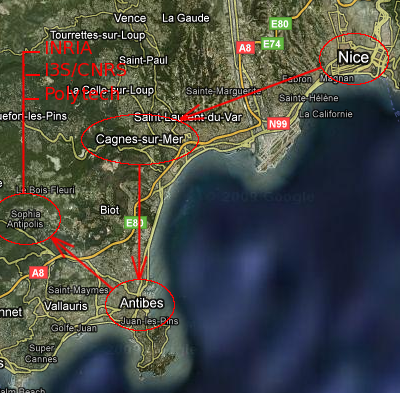
\includegraphics[scale=0.7]{img/screenshot/geolock2}\\

Un ingénieur expert souhaite, pour réduire le coup de son trajet journalier, faire du co-voiturage. Il décide alors de publier une proposition de covoiturage dans son réseau P2P:\\ 

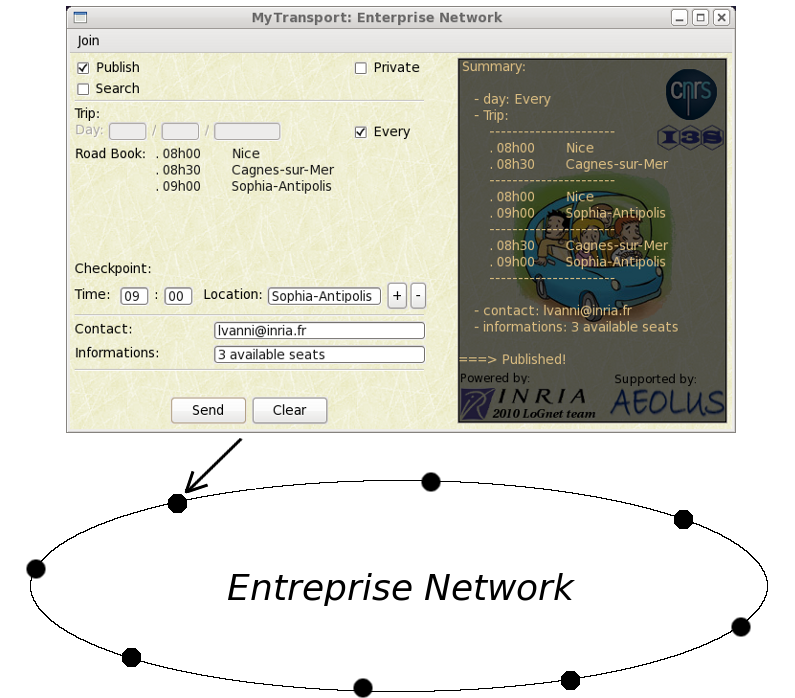
\includegraphics[scale=0.6]{img/screenshot/enterprisePub}\\

Les différents champs que nous voyons ici représentent plusieurs valeurs associées a plusieurs clefs, explications:\\
Tout d'abord, la partie Trip:
\begin{itemize}
\item Le premier champ concerne la date à laquelle le trajet va être effectué: L'utilisateur peut soit saisir la date soit cocher la checkBox "Every" qui permet de préciser qu'il s'agit d'un trajet journalier.
\item La deuxième partie (Road Book), permet d'enregistrer l'itinéraire prévu:
			\begin{itemize}
			\item 08h00 Nice
			\item 08h30 Cagnes-sur-Mer
			\item 09h00 Sophia-Antipolis
			\end{itemize}
\end{itemize}
Cette partie permet de créer toutes les clefs correspondant à tous les itinéraires possible:
\begin{itemize}
\item Clef 1 : Nice 08h00 | Cagnes-sur-Mer 08h30 | Every days
\item Clef 2 : Nice 08h00 | Sophia-Antipolis 09h00 | Every days
\item Clef 3 : Cagnes-sur-Mer 08h30 | Sophia-Antipolis 09h00 |  | Every days \\ ~ \\
\end{itemize}

La deuxième partie, constitue la valeur associée a chacune de ces clefs. Cette valeur est la concaténation des informations:
\begin{itemize}
\item Contact = Nom de la personne concernée, email, téléphone, ...
\item Informations = Toutes informations utiles (Nombre de place, type de voiture, ...) \\
\end{itemize}

Cette proposition de co-voiturage va donc être visible de tous les membres non étudiants des trois centres de recherches. Un utilisateur cherchant donc une proposition de co-voiturage entre Nice et Sophia-Antipolis obtiendra:\\

~ 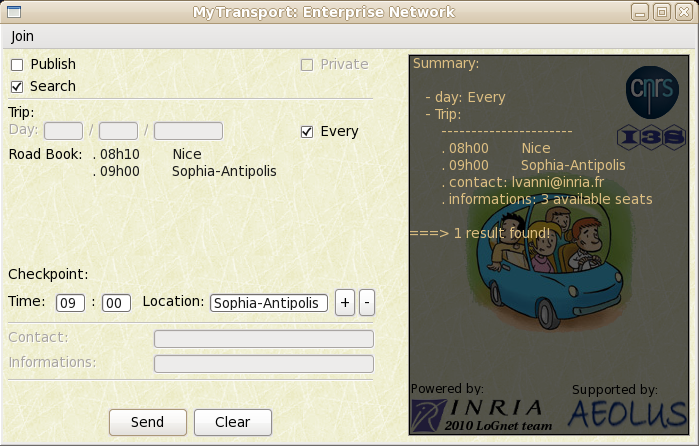
\includegraphics[scale=0.55]{img/screenshot/NiceSophiaSub}\\

Un autre aspect de cette application, est qu'il possible de réunir plusieurs itinéraires déjà publiés pour les combiner et en faire d'autres pour répondre à plus de demandes:

~ 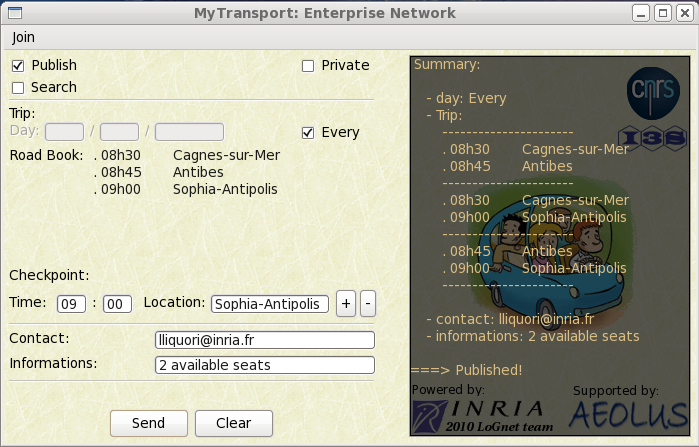
\includegraphics[scale=0.55]{img/screenshot/CagnesAntibesSophiaPub}\\

Ici on peut voir un utilisateur qui publie un nouvel itinéraire avec cette fois-ci Antibes en point de passage.\\

Supposons maintenant qu'un autre utilisateur souhaite faire le trajet:
\begin{itemize}
\item 08h00 Nice
\item 08h30 Cagnes-sur-Mer
\item 08h45 Antibes \\
\end{itemize}

~ 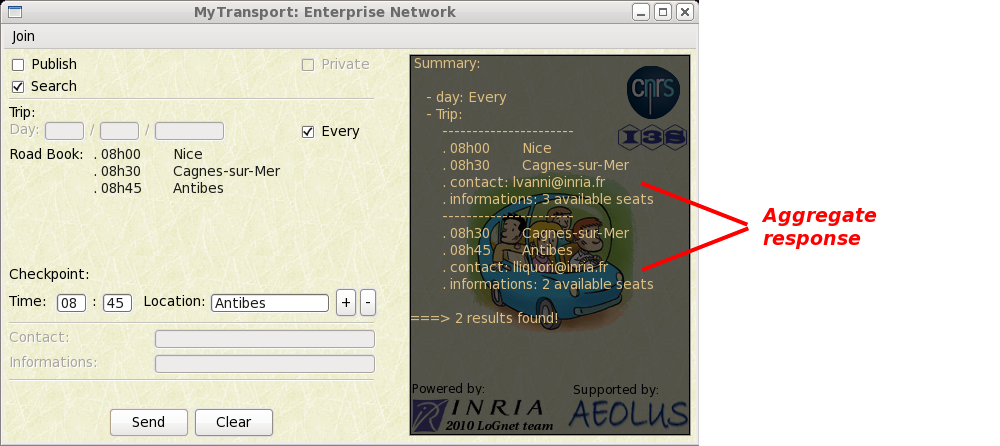
\includegraphics[scale=0.50]{img/screenshot/NiceCagnesAntibesSub}\\

Nous voyons ici que la requête issue de la demande à permis de générer un résultat composer de plusieurs propositions de covoiturage différentes.\\ ~ \\

L'ingénieur expert peut ainsi profiter du système de co-voiturage avec ces collègues des différents centres de recherches de Sophia-Antipolis. Malgré cela, il reste encore des places disponibles dans sa voiture pour son trajet quotidien. Pour optimiser encore plus l'utilisation de sa voiture, il souhaiterai maintenant partager ses informations avec les étudiants qui disposent de leur propre réseaux de co-voiturage (ici identique au niveau du fonctionnement).\\

~ 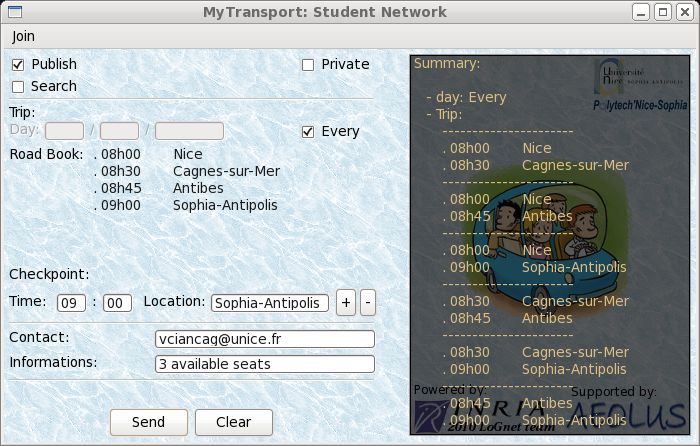
\includegraphics[scale=0.55]{img/screenshot/NiceCagnesAbtibesSophiaPub_studentNetwork}\\

Pour cela on une checkBox "private" , qui permet de préciser si l'on souhaite rendre ces informations publique (c'est a dire qu'elles soit visible depuis d'autres réseaux) ou pas.
Cette seule indication ne suffit pas a diffuser l'information en dehors du réseaux, les deux réseaux de notre exemple étant hétérogènes et a priori non collaboratifs. Pour y parvenir nous allons maintenant introduire le concept de Synapse, dont le but est d'inter-connecter ce genre de réseaux.

 
\clearpage

%---------------------------
% Synapse
%---------------------------
\section{Synapse}
Les Synapse sont des pairs, qui appartiennent a plusieurs réseaux P2P en même temps. Dans notre exemple ont peut associer cette propriété a un type d'étudiant particulier: \textbf{Les apprentis et les stagiaires.} \\

Le cursus universitaire propose aujourd'hui aux étudiants d'effectuer des stages en entreprise ou même de valider des années en alternances en partageant l'emploi du temps entre l'université et l'entreprise. Ainsi chaque année, l'INRIA accueil des étudiants qui côtoient les chercheurs, enseignants, doctorants et autres ingénieurs experts... 
Ces étudiants remplissent toutes les caractéristiques des synapses, ils appartiennent a la fois au réseau Etudiant et au réseau Entreprise. Dans notre application, ce double statu leur permet d'accéder aux deux réseaux de co-voiturage (avec la même interface). C'est un mécanisme d'invitations similaire aux réseaux sociaux privés qui leur permet de joindre un nouveau réseau. A noter que ce mécanisme n'est pas réservé aux apprentis et aux stagiaires, mais permet a n'importe quel autre membre d'un réseau de devenir synapse, s'il dispose d'une invitation vers un autre réseau.\\

~~~~~~~~~~~~~~~~~~~~~~~~~~~~~ 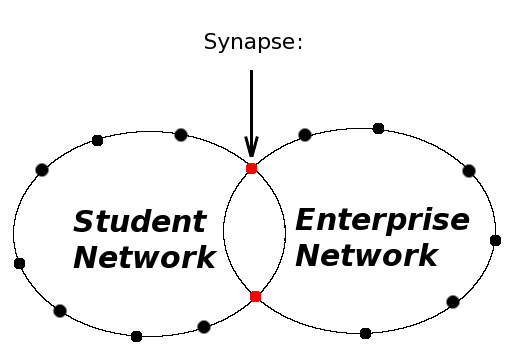
\includegraphics[scale=0.4]{img/schema/Synapse}\\

Les synapses servent de connexion entre ces réseaux hétérogènes. Le protocole décrit précédemment permet de diffuser et de partager les informations entre les différents réseaux. Pour notre application de co-voiturage, le champ "plublic" permet donc de spécifier si l'on souhaite que les informations soit visible ou pas depuis d'autres réseaux.\\
\clearpage
Pour conclure avec notre exemple de l'ingénieur expert qui souhaite faire du co-voiturage, nous voyons que les informations qu'il a publié dans son réseau Entreprise son maintenant visible depuis le réseau Etudiant. Les membres du réseaux Etudiant bénéficient en fait d'une ou plusieurs synapses qui leur permet de propager leurs requêtes de réseaux en réseaux. \\

~~~~~~~~~~~~~~~~~~~~~~~~~~~~~ 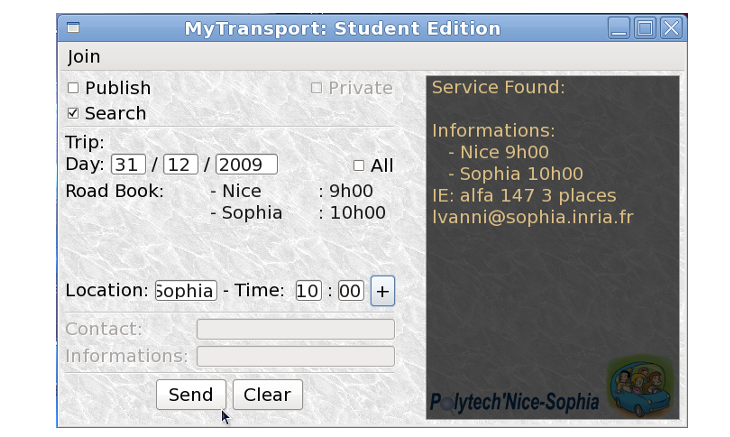
\includegraphics[scale=0.4]{img/screenshot/studentSubFound}\\
 
\clearpage

%---------------------------
% Perspective et Évolution
%---------------------------
\section{Perspectives et Évolutions}
Ce système d'overlay robuste permet de couvrir de manière quasi optimal une zone géographique en co-voiturage. De plus la scalabilité du modèle P2P permet d'envisager d'étendre ce modèle sur toute une région ou même plus, en ajoutant de nouveaux réseaux liés a d'autres entreprises et en faisant apparaitre de nouvelles synapses. Le protocole synapse permet d'interconnecter n'importe quels réseaux, il suffit donc de créer de nouveaux réseaux de covoiturage, spécialisé et adapté a une zone géographique ou a des entreprises pour optimiser le covoiturage entre eux.\\

D'un point de vue technique l'utilisation de réseaux pair a pair permet d'envisager simplement l'ajout de nouveaux services:\\
Par exemple, pour nos réseaux Student et Enterprise, on pourrai imaginer de mettre au point un service de transfère de fichiers/données. Le P2P, très adapté a ce genre de services (plusieurs protocole comme bittorrent) permettrai dans notre cas d'autoriser l'échange de données entre les chercheurs, ingénieurs et professeurs des 3 centres de recherches. Les étudiants de leur coté pourrai aussi s'échanger des données tout en bénéficiant de certains cours ou papier mis a disposition par le réseau entreprise.\\

On pourrait aussi imaginer d'intégrer des systèmes (géolocalisation GPS, RFID) permettant de mettre automatiquement a jour le statu d'un utilisateur suivant sa position géographique. Un système de notification SMS pourrait être mis en place lorsqu'un utilisateur décide de rentrer chez lui pour ameliorer encore plus le système de covoiturage dans le cas des horaires flexibles.




 
\clearpage

%---------------------------
% Conclusion
%---------------------------
\section{Conclusion}
%\textbf{Pré-requis:} Ce prototype ne prend pas en compte le \% de personnes utilisant les transports en communs.\\

Considérons trois centres de recherches et développements géographiquement très proches:
\begin{itemize}
\item L'école Polytech'Nice-Sophia
\item L'INRIA - Sophia Antipolis - Méditerranée , France
\item Le laboratoire i3s du CNRS \\
\end{itemize}

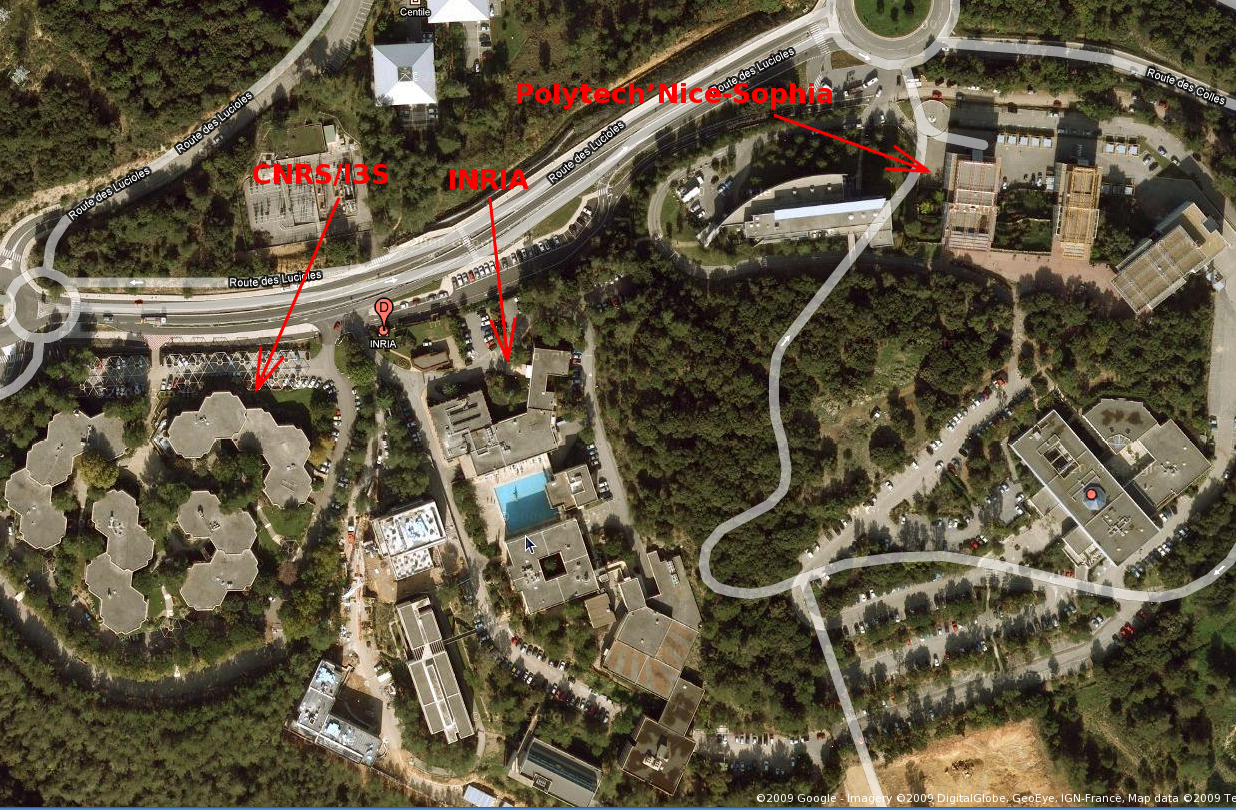
\includegraphics[scale=0.35]{img/screenshot/geolock} \\

Parmi ces 3 centres, on peut distinguer 2 types de personnes:
\begin{itemize}
\item Les Étudiants: \\
	Polytech'Nice-Sophia accueille près de \textbf{1.000 élèves} qui suivent les formations offertes dans cinq grands domaines scientifiques et technologiques  - Électronique, Informatique, Mathématiques appliquées, Génie biologique et Ingénierie de l'eau
\item Les Autres: \\
	Chercheurs, enseignants chercheurs, doctorant, ingénieurs, personnels administratifs, ...)
	repartis entre l'INRIA, le CNRS et l'école Polytech'Nice-Sophia (\textbf{environs 500 personnes}) \\
\end{itemize} 

Le cas critique pour cette zone géographique de sophia-antipolis, serai que toutes ces personnes possèdent une voiture sans jamais faire de covoiturage: environs 1500 voitures mobilisées tous les jours!
A l'inverse, le cas idéal serai que tout le monde propose de faire du co-voiturage, on obtiendrait pour 4 places disponibles par voiture:
1500/4 = 375 voitures mobilisées par jours, ce qui équivaut a une baisse de 75\% \\

Le but est donc ici d'optimiser au maximum le co-voiturage dans cette zone pour s'approcher le plus possible du cas idéal. 




 
\clearpage

\end{document}


